\documentclass[12pt,a4paper]{article}
\usepackage[hidelinks]{hyperref}
\usepackage{fancyhdr} % برای هدر/فوتر سفارشی
\usepackage{titlesec} % برای قالب‌بندی بخش‌ها
\usepackage{epsfig,graphicx,subfigure,amsthm,amsmath}
\usepackage{color,xcolor}
\usepackage{xepersian}
\usepackage{setspace}
\settextfont[Scale=1.2]{XB Niloofar}
\setlatintextfont[Scale=1]{Times New Roman}

% عنوان و اطلاعات نویسنده
\title{کاربرد موجک در معادلات انتگرالی الکترومغناطیسی}
\author{محمد مهدی الیاسی \\ استاد: دکتر مرادی}
\date{۴ بهمن ۱۴۰۳}

\begin{document}

% صفحه عنوان با نماد دانشگاه
\begin{center}
    
\includegraphics[width=0.3\textwidth]{amirkabir.png} \\[2em]
    
    \LARGE \textbf{بررسی تبدیل ملین: ویژگی‌ها، مثال‌ها و کاربردها} \\[1em]
    \large \textbf{نویسنده: محمد مهدی الیاسی} \\[1em]
    \large \textbf{استاد: دکتر مرادی}\\[1em]
    \large \textbf{درس: ریاضیات مهندسی پیشرفته} \\[4em]
    \large \textbf{دانشکده مهندسی برق} \\[4em]
\end{center}

% تاریخ در پایین صفحه
\vfill
\begin{center}
    \large \today
\end{center}

\newpage

% فهرست مطالب
\tableofcontents
\newpage

% Introduction
\section{مقدمه}
تبدیل ملین یک ابزار ریاضی انعطاف‌پذیر است که نقش حیاتی در حل مسائل مختلف در ریاضیات، فیزیک و مهندسی ایفا می‌کند\cite{Mellin}. این تبدیل به عنوان یک تبدیل انتگرالی، روشی منحصربه‌فرد برای تحلیل توابع از طریق نگاشت آن‌ها به حوزه مختلط فراهم می‌کند. این تبدیل به‌ویژه در مطالعه رفتارهای مجانبی ارزشمند است و در زمینه‌هایی مانند تحلیل مجانبی، نظریه اعداد و مکانیک کوانتوم ضروری است. در مهندسی، این تبدیل در پردازش سیگنال و تحلیل تصاویر کاربرد دارد، جایی که تکنیک‌های حوزه فرکانس برای تفسیر داده‌ها ضروری هستند.

اهمیت تبدیل ملین در توانایی آن برای ساده‌سازی پردازش‌های ضربی و رفتارهای قانون توان نهفته است. با تبدیل توابع تعریف‌شده در دامنه واقعی مثبت به فرمی ساده‌تر، تحلیل و محاسبه آن‌ها راحت‌تر می‌شود.

این گزارش قصد دارد ویژگی‌های تبدیل ملین را بررسی کرده و مبانی نظری آن را از طریق مثال‌های عملی تأیید کند. با استفاده از پایتون به عنوان یک ابزار محاسباتی، تبدیل‌ها به صورت عددی محاسبه می‌شوند، هویت‌های ریاضی تأیید می‌شوند و نتایج به صورت گرافیکی نمایش داده می‌شوند. جنبه‌های کلیدی مانند ویژگی‌های مقیاس‌بندی، انتقال و کاربردهای خاص به منظور ارائه یک درک جامع از این ابزار قدرتمند ریاضی نشان داده خواهند شد.

\section{پیش‌زمینه ریاضی}
تبدیل ملین یک تابع $f(x)$ به صورت زیر تعریف می‌شود:
\begin{equation}
\mathcal{M}\{f(x)\}(s) = \int_{0}^{\infty} x^{s-1} f(x) \, dx,
\end{equation}
که در آن $s = \sigma + i\omega$ یک متغیر مختلط است. این تبدیل یک تابع $f(x)$ تعریف‌شده در دامنه مثبت واقعی را به صفحه مختلط نگاشت می‌کند و برای تحلیل مسائل شامل ویژگی‌های مقیاس‌ناپذیر و ساختارهای ضربی مفید است.

یک حالت خاص از تبدیل ملین زمانی است که $f(x) = e^{-x}$ باشد، که منجر به تابع گاما می‌شود:
\begin{equation}
\Gamma(s) = \int_{0}^{\infty} x^{s-1} e^{-x} \, dx.
\end{equation}
تابع گاما نقش حیاتی در تبدیل ملین ایفا می‌کند زیرا راه‌حل‌های بسته برای توابع خاص فراهم می‌آورد و به عنوان یک بلوک سازنده برای بسیاری از نتایج تحلیلی استفاده می‌شود. این تابع در نظریه احتمالات، ترکیبیات و تحلیل مختلط به طور گسترده‌ای استفاده می‌شود.

تبدیل ملین ویژگی‌های مهمی دارد:
\begin{itemize}
    \item \textbf{ویژگی انتقال:} اگر $f(x)$ به صورت $x^a f(x)$ تبدیل شود، آنگاه:
    \begin{equation}
    \mathcal{M}\{x^a f(x)\}(s) = \mathcal{M}\{f(x)\}(s + a).
    \end{equation}
    \item \textbf{ویژگی مقیاس‌بندی:} اگر $f(x)$ به صورت $f(ax)$ مقیاس‌بندی شود، آنگاه:
    \begin{equation}
    \mathcal{M}\{f(ax)\}(s) = a^{-s} \mathcal{M}\{f(x)\}(s).
    \end{equation}
    \item \textbf{ارتباط با تابع گاما:} برای توابعی مانند $e^{-x}$، تبدیل ملین مستقیماً به تابع گاما تبدیل می‌شود.
\end{itemize}

این ویژگی‌ها تبدیل ملین را به ابزاری قدرتمند برای حل مسائل شامل معادلات دیفرانسیل، رفتارهای مجانبی و انتگرال‌ها تبدیل می‌کند. بخش‌های بعدی گزارش این ویژگی‌ها و کاربردهای آن‌ها را از طریق محاسبات عددی نشان می‌دهند.

\section{اثبات تبدیل ملین برای $f(x) = e^{-x}$}
تبدیل ملین تابع نمایی $f(x) = e^{-x}$ یک مثال کلاسیک است که ارتباط آن با تابع گاما را نشان می‌دهد. به صورت ریاضی، این تبدیل عبارت است از:
\begin{equation}
\mathcal{M}\{e^{-x}\}(s) = \int_{0}^{\infty} x^{s-1} e^{-x} \, dx = \Gamma(s).
\end{equation}
این انتگرال برای $\Re(s) > 0$ همگرا است، جایی که $\Gamma(s)$ نشان‌دهنده تابع گاما است که به طور گسترده در ریاضیات و علوم استفاده می‌شود.

برای تأیید این نتیجه، از پایتون برای محاسبه عددی تبدیل ملین و مقایسه آن با تابع گامای تحلیلی استفاده کردیم\cite{Code}.

\subsection{پیاده‌سازی در پایتون}
کد پایتون زیر برای محاسبه عددی تبدیل ملین $f(x) = e^{-x}$ استفاده شد:
\begin{verbatim}
import numpy as np
import scipy.integrate as integrate
from scipy.special import gamma
import matplotlib.pyplot as plt

# Define Mellin transform for f(x) = e^(-x)
def mellin_transform(f, p):
    return integrate.quad(lambda x: x**(p-1) * f(x), 0, np.inf)[0]

# Define the exponential function
def f(x):
    return np.exp(-x)

# Generate p values
p_values = np.linspace(0.1, 5, 100)

# Compute values
gamma_vals = gamma(p_values)
mt_vals = [mellin_transform(f, p) for p in p_values]

# Plot results
plt.figure(figsize=(10, 6))
plt.plot(p_values, gamma_vals, 'b-', label='Analytical Gamma Function')
plt.plot(p_values, mt_vals, 'r--', label='Numerical Mellin Transform')
plt.xlabel('p')
plt.ylabel('Value')
plt.title('Mellin Transform of $f(x) = e^{-x}$')
plt.legend()
plt.grid(True)
plt.show()
\end{verbatim}

\subsection{نتایج و مقایسه}
نتایج محاسبات عددی در کنار تابع گامای تحلیلی ترسیم شدند، همانطور که در زیر نشان داده شده است:

\begin{figure}[H]
    \centering
    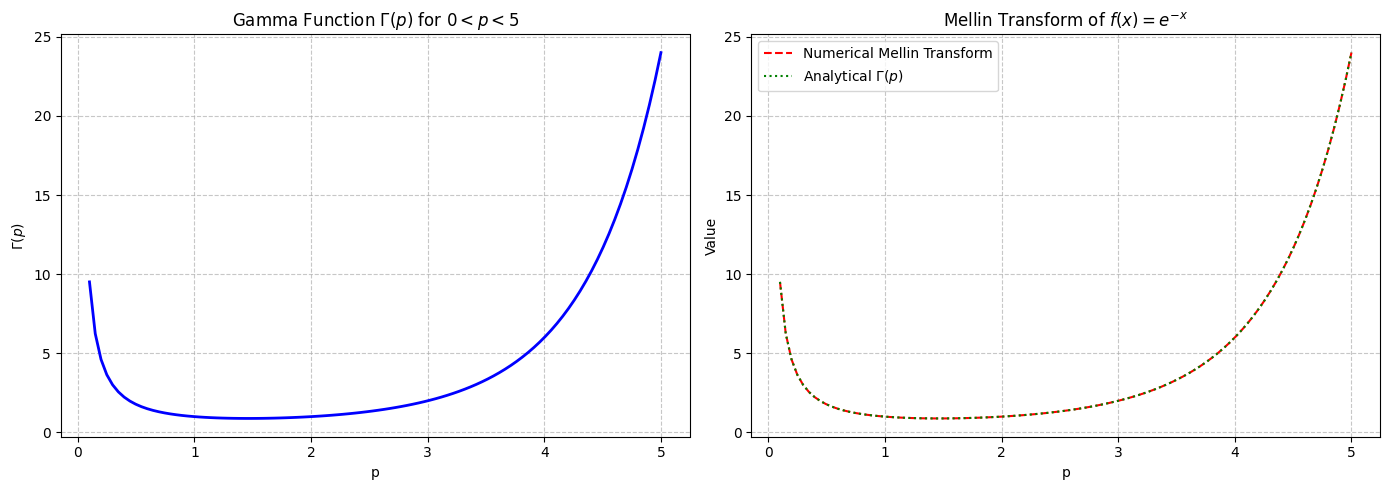
\includegraphics[width=0.8\textwidth]{Prooving Gamma function.png}
    \caption{مقایسه تبدیل ملین عددی و تابع گامای تحلیلی برای $f(x) = e^{-x}$.}
    \label{fig:gamma_vs_mellin}
\end{figure}

این نمودار تطابق عالی بین نتایج عددی و تحلیلی را نشان می‌دهد و ارتباط بین تبدیل ملین برای $f(x) = e^{-x}$ و تابع گاما را تأیید می‌کند.
\section{تأیید تبدیل ملین برای $f(x) = \frac{1}{x+1}$}

تابع $f(x) = \frac{1}{x+1}$ به عنوان یک مثال دیگر برای بررسی تبدیل ملین عمل می‌کند. تبدیل ملین مربوط به این تابع به صورت زیر است:
\begin{equation}
\int_{0}^{\infty} \frac{x^{p-1}}{x+1} \, dx = \frac{\pi}{\sin(\pi p)}.
\end{equation}
این هویت انتگرالی ارتباط بین تبدیل ملین و توابع مثلثاتی را نشان می‌دهد.

\subsection{ارتباط با توابع گاما}
هویت فوق همچنین می‌تواند با استفاده از تابع گاما به صورت زیر بیان شود:
\begin{equation}
\Gamma(p) \Gamma(1-p) = \frac{\pi}{\sin(\pi p)}.
\end{equation}
این رابطه تعامل بین تبدیل ملین و تابع گاما را نشان می‌دهد و اهمیت تحلیلی آن را تقویت می‌کند.

\subsection{پیاده‌سازی در پایتون}
کد پایتون زیر برای محاسبه عددی تبدیل ملین، ارزیابی حاصل‌ضرب گاما و مقایسه نتایج با راه‌حل تحلیلی استفاده شد:
\begin{verbatim}
import numpy as np
from scipy.special import gamma
import matplotlib.pyplot as plt
from scipy.integrate import quad

# Define the function
f = lambda x: 1 / (x + 1)

# Define Mellin Transform for f(x)
def mellin_transform(f, p):
    result, _ = quad(lambda x: x**(p-1) * f(x), 0, np.inf)
    return result

# Generate p values
p_values = np.linspace(0.1, 0.9, 100)

# Compute values
mt_values = [mellin_transform(f, p) for p in p_values]
gamma_product = [gamma(p) * gamma(1 - p) for p in p_values]
analytical = [np.pi / np.sin(np.pi * p) for p in p_values]

# Plot results
plt.figure(figsize=(10, 6))
plt.plot(p_values, mt_values, 'b-', label='Numerical Mellin Transform')
plt.plot(p_values, gamma_product, 'g--', label='Gamma Product')
plt.plot(p_values, analytical, 'r:', label='Analytical Solution')
plt.xlabel('p')
plt.ylabel('Value')
plt.title('Verification of Mellin Transform for $f(x) = \\frac{1}{x+1}$')
plt.legend()
plt.grid(True)
plt.show()
\end{verbatim}

\subsection{نتایج و بصری‌سازی}
نتایج حاصل از محاسبه عددی، حاصل‌ضرب گاما و راه‌حل تحلیلی ترسیم و مقایسه شدند. نمودار زیر نشان می‌دهد که این مقادیر تا چه اندازه با هم مطابقت دارند:

\begin{figure}[H]
    \centering
    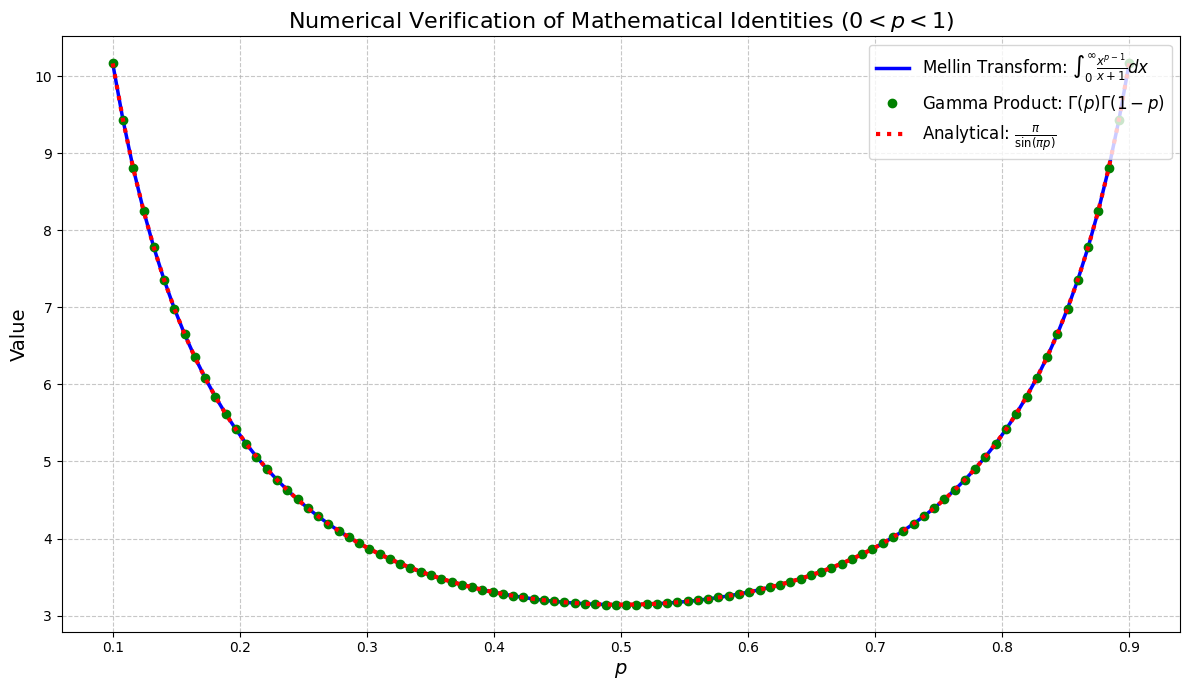
\includegraphics[width=0.8\textwidth]{Example.png}
    \caption{تأیید عددی هویت‌های ریاضی برای $f(x) = \frac{1}{x+1}$ ($0 < p < 1$).}
    \label{fig:mellin_identity}
\end{figure}

تطابق بین نتایج عددی، حاصل‌ضرب گاما و راه‌حل تحلیلی هویت نظری را تأیید می‌کند. این مثال بر کاربرد تبدیل ملین در تحلیل توابع و تأیید هویت‌های ریاضی تأکید می‌کند.
\section{بررسی ویژگی‌های مقیاس‌بندی و انتقال}

ویژگی‌های مقیاس‌بندی و انتقال در تبدیل ملین اطلاعاتی درباره رفتار توابع تحت تبدیل‌ها ارائه می‌دهند. این ویژگی‌ها در ادامه تعریف شده و به صورت عددی بررسی می‌شوند.

\subsection{ویژگی مقیاس‌بندی}
ویژگی مقیاس‌بندی تبدیل ملین بیان می‌کند:
\begin{equation}
\mathcal{M}\{f(ax)\}(s) = a^{-s} \mathcal{M}\{f(x)\}(s),
\end{equation}
که در آن $a > 0$ است. این ویژگی نشان می‌دهد که مقیاس‌بندی آرگومان تابع منجر به یک ضریب ضربی در دامنه تبدیل می‌شود.

\subsection{ویژگی انتقال}
ویژگی انتقال تبدیل ملین به صورت زیر تعریف می‌شود:
\begin{equation}
\mathcal{M}\{x^a f(x)\}(s) = \mathcal{M}\{f(x)\}(s + a).
\end{equation}
این ویژگی توصیف می‌کند که چگونه ضرب تابع در یک توان از $x$ باعث انتقال آرگومان تبدیل می‌شود.

\subsection{پیاده‌سازی در پایتون}
کد پایتون زیر تأیید عددی هر دو ویژگی را نشان می‌دهد:
\begin{verbatim}
import numpy as np
from scipy.integrate import quad
from scipy.special import gamma
import matplotlib.pyplot as plt

# Define Mellin transform function
def mellin_transform(f, p):
    result, _ = quad(lambda x: x**(p-1) * f(x), 0, np.inf)
    return result

# Define original and transformed functions
def f(x):
    return np.exp(-x)

def scaled_f(x, a):
    return f(a * x)

def shifted_f(x, a):
    return x**a * f(x)

# Parameters
a = 2
p_values = np.linspace(0.1, 5, 100)

# Compute values for scaling
scaling_numerical = [mellin_transform(lambda x: scaled_f(x, a), p) for p in p_values]
scaling_analytical = [a**-p * mellin_transform(f, p) for p in p_values]

# Compute values for shifting
shifting_numerical = [mellin_transform(lambda x: shifted_f(x, a), p) for p in p_values]
shifting_analytical = [mellin_transform(f, p + a) for p in p_values]

# Plot results
plt.figure(figsize=(12, 6))

# Scaling
plt.subplot(1, 2, 1)
plt.plot(p_values, scaling_numerical, 'bo', label='Numerical Scaling')
plt.plot(p_values, scaling_analytical, 'r--', label='Analytical Scaling')
plt.title(f'Scaling Property: $f(ax)$, $a = {a}$')
plt.xlabel('$s$')
plt.ylabel('Value')
plt.legend()

# Shifting
plt.subplot(1, 2, 2)
plt.plot(p_values, shifting_numerical, 'mo', label='Numerical Shifting')
plt.plot(p_values, shifting_analytical, 'g--', label='Analytical Shifting')
plt.title(f'Shifting Property: $x^a f(x)$, $a = {a}$')
plt.xlabel('$s$')
plt.ylabel('Value')
plt.legend()

plt.tight_layout()
plt.show()
\end{verbatim}

\subsection{نتایج و بصری‌سازی}
نتایج تأیید عددی هر دو ویژگی در زیر نشان داده شده است:

\begin{figure}[H]
    \centering
    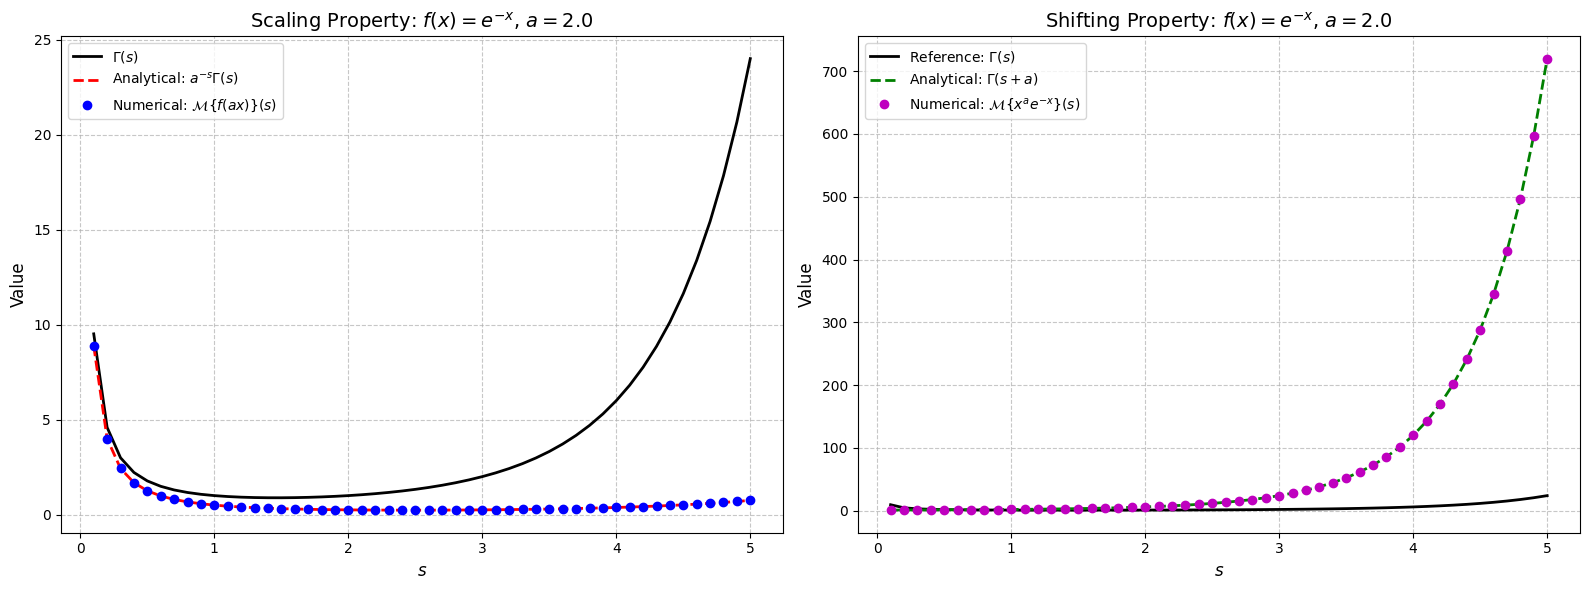
\includegraphics[width=0.8\textwidth]{Shifting and scaling.png}
    \caption{تأیید عددی ویژگی‌های مقیاس‌بندی و انتقال برای $f(x) = e^{-x}$.}
    \label{fig:scaling_shifting}
\end{figure}

نمودارها تطابق بین نتایج عددی و عبارات تحلیلی را تأیید می‌کنند و ویژگی‌های مقیاس‌بندی و انتقال تبدیل ملین را معتبر می‌سازند.
\section{بصری‌سازی $\phi(r, \theta)$}

تابع $\phi(r, \theta)$ با استفاده از یک روش کانولوشنی محاسبه می‌شود که در آن انتگرالی بر روی تابع $f(\xi)$ با وزنده تابع دیگری $h(r/\xi, \theta)$ انجام می‌گیرد. این به صورت ریاضی به شکل زیر تعریف می‌شود:
\begin{equation}
\phi(r, \theta) = \int_{0}^{\infty} f(\xi) \frac{h(r/\xi, \theta)}{\xi} \, d\xi.
\end{equation}

\subsection{نقش $h(r, \theta)$ و $f(\xi)$}
- تابع $h(r, \theta)$ به عنوان یک هسته عمل می‌کند که تابع ورودی $f(\xi)$ را بر اساس پارامترهای $r$ و $\theta$ مدوله می‌کند. این تابع اطلاعاتی درباره رابطه بین مقیاس $r$ و زاویه $\theta$ کدگذاری می‌کند.
- تابع $f(\xi)$ سیگنال یا داده ورودی را نمایش می‌دهد که با هسته $h(r, \theta)$ کانولوشن شده و خروجی $\phi(r, \theta)$ را تولید می‌کند.

\subsection{پیاده‌سازی در پایتون}
کد پایتون زیر محاسبه $\phi(r, \theta)$ را نشان می‌دهد:
\begin{verbatim}
import numpy as np
from scipy.integrate import quad
import matplotlib.pyplot as plt

# Define h(r, theta)
def h_function(r, theta, alpha):
    n = np.pi / (2 * alpha)
    term1 = (r**n) * (1 + r**(2 * n)) * np.cos(n * theta)
    term2 = 1 + 2 * r**(2 * n) * np.cos(2 * n * theta) + r**(4 * n)
    return term1 / term2

# Define phi(r, theta)
def phi_function(r, theta, alpha, f):
    def integrand(xi):
        h_val = h_function(r / xi, theta, alpha)
        return f(xi) * h_val / xi
    return quad(integrand, 0, np.inf, limit=50)[0]

# Example f(xi)
def f_function(xi):
    return np.exp(-xi)

# Define range for theta and r
alpha = np.pi / 4
theta_values = np.linspace(-alpha, alpha, 50)
r_values = np.linspace(0.1, 5, 50)

# Compute phi(r, theta)
phi_values = np.zeros((len(r_values), len(theta_values)))
for i, r in enumerate(r_values):
    for j, theta in enumerate(theta_values):
        phi_values[i, j] = phi_function(r, theta, alpha, f_function)

# Plot results
R, THETA = np.meshgrid(r_values, theta_values)
plt.figure(figsize=(10, 6))
plt.contourf(R, THETA, phi_values.T, levels=50, cmap='viridis')
plt.colorbar(label='$\\phi(r, \\theta)$')
plt.title('$\\phi(r, \\theta)$ for $\\theta \\in [-\\pi/4, \\pi/4]$ and $r \\in [0.1, 5]$')
plt.xlabel('r')
plt.ylabel('$\\theta$')
plt.show()
\end{verbatim}

\subsection{نتایج و بصری‌سازی}
نمودار کانتور $\phi(r, \theta)$ در زیر نشان داده شده است:

\begin{figure}[H]
    \centering
    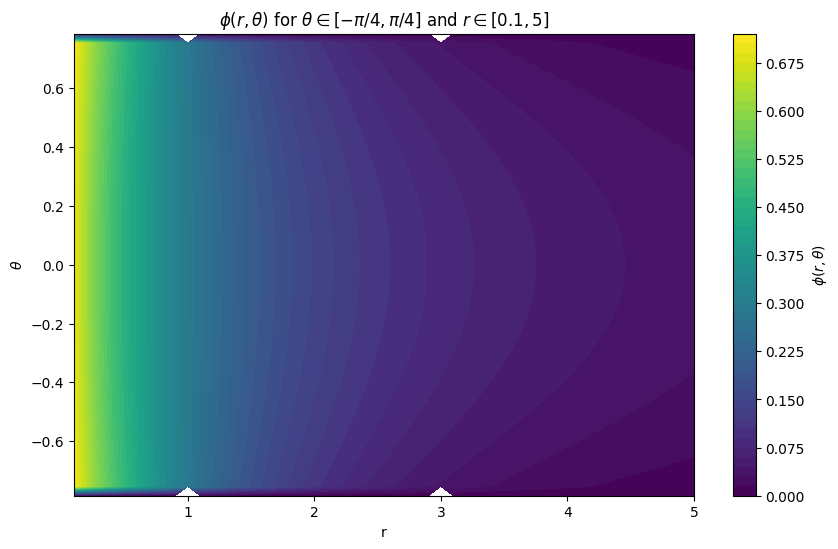
\includegraphics[width=0.8\textwidth]{Phi.png}
    \caption{نمودار کانتور $\phi(r, \theta)$ برای $\theta \in [-\pi/4, \pi/4]$ و $r \in [0.1, 5]$.}
    \label{fig:phi_contour}
\end{figure}

این بصری‌سازی تغییرات $\phi(r, \theta)$ را نسبت به پارامترهای $r$ و $\theta$ نشان می‌دهد. نتایج تأثیر هسته $h(r, \theta)$ و تابع ورودی $f(\xi)$ بر خروجی را برجسته می‌کند.

\section{نتیجه‌گیری}
تبدیل ملین به عنوان ابزاری قدرتمند برای تحلیل توابع نشان داده شده است که راهی منحصربه‌فرد برای مطالعه ویژگی‌های مقیاس‌ناپذیر و فرایندهای ضربی ارائه می‌دهد. این گزارش هویت‌ها و ویژگی‌های کلیدی مانند مقیاس‌بندی، انتقال و محاسبات مبتنی بر کانولوشن را تأیید کرد. پیاده‌سازی‌های عددی و تطابق آن‌ها با نتایج تحلیلی قابلیت اطمینان پایتون را برای تحلیل ریاضی نشان می‌دهند.

پیشنهادات برای گسترش این کار شامل موارد زیر است:
\begin{itemize}
    \item بررسی تبدیل ملین در ابعاد بالاتر برای تحلیل توابع چندمتغیره.
    \item استفاده از تبدیل ملین در علم داده، مانند استخراج ویژگی‌ها و تجزیه سیگنال.
    \item بررسی نقش آن در حل معادلات دیفرانسیل پیشرفته و معادلات انتگرالی.
\end{itemize}
\newpage

\clearpage

\section{مراجع}

\begin{thebibliography}{99}
    \bibitem{Mellin} Debnath, Lokenath, and Dambaru Bhatta.\textit{l Transforms and Their Applications. 2nd ed.},CRC Press, 1995.
    \bibitem{Code} Github link,\textit{Mellin-transform} at \url{https://github.com/MohammadMahdiElyasi/Mellin-transform}.

\end{thebibliography}

\end{document}